% -----------------------------------------------------------------------
% outputs.tex: Section detailing the different forms of text- and
%              plot-based output.
% -----------------------------------------------------------------------
% Copyright (C) 2006, Matthew Whiting, ATNF
%
% This program is free software; you can redistribute it and/or modify it
% under the terms of the GNU General Public License as published by the
% Free Software Foundation; either version 2 of the License, or (at your
% option) any later version.
%
% Duchamp is distributed in the hope that it will be useful, but WITHOUT
% ANY WARRANTY; without even the implied warranty of MERCHANTABILITY or
% FITNESS FOR A PARTICULAR PURPOSE.  See the GNU General Public License
% for more details.
%
% You should have received a copy of the GNU General Public License
% along with Duchamp; if not, write to the Free Software Foundation,
% Inc., 59 Temple Place, Suite 330, Boston, MA 02111-1307, USA
%
% Correspondence concerning Duchamp may be directed to:
%    Internet email: Matthew.Whiting [at] atnf.csiro.au
%    Postal address: Dr. Matthew Whiting
%                    Australia Telescope National Facility, CSIRO
%                    PO Box 76
%                    Epping NSW 1710
%                    AUSTRALIA
% -----------------------------------------------------------------------
\secA{Outputs}
\label{sec-output}

\secB{During execution}
 
\duchamp provides the user with feedback whilst it is running, to
keep the user informed on the progress of the analysis. Most of this
consists of self-explanatory messages about the particular stage the
program is up to. The relevant parameters are printed to the screen at
the start (once the file has been successfully read in), so the user
is able to make a quick check that the setup is correct (see
Appendix~\ref{app-input} for an example).

The extent of memory allocation made at the start is indicated. This
will include the arrays needed for the pixel array, the reconstruction
or smoothed array, and the 2D detection map, but \emph{not} additional
space needed for working within individual algorithms, nor storage
needed for the detected objects.

\duchamp will report the amount of memory that is allocated when the
image is read in. This includes the storage for the array as well as
additional storage for the reconstructed/smoothed array and/or the
baseline arrays (if these are needed).

If the cube is being trimmed (\S\ref{sec-modify}), the resulting
dimensions are printed to indicate how much has been trimmed. If a
reconstruction is being done, a continually updating message shows
either the current iteration and scale, compared to the maximum scale
(when \texttt{reconDim = 3}), or a progress bar showing the amount of
the cube that has been reconstructed (for smaller values of
\texttt{reconDim}).

During the searching algorithms, the progress through the search is
shown. When completed, the number of objects found is reported (this
is the total number found, before any merging is done).

In the merging process (where multiple detections of the same object
are combined -- see \S\ref{sec-merger}), two stages of output
occur. The first is when each object in the list is compared with all
others. The output shows two numbers: the first being how far through
the list the current object is, and the second being the length of the
list. As the algorithm proceeds, the first number should increase and
the second should decrease (as objects are combined). When the numbers
meet, the whole list has been compared. If the objects are being
grown, a similar output is shown, indicating the progress through the
list. In the rejection stage, in which objects not meeting the minimum
pixels/channels requirements are removed, the total number of objects
remaining in the list is shown, which should steadily decrease with
each rejection until all have been examined. Note that these steps can
be very quick for small numbers of detections.

Since this continual printing to screen has some overhead of time and
CPU involved, the user can elect to not print this information by
setting the parameter \texttt{verbose = false}. In this case, the user
is still informed as to the steps being undertaken, but the details of
the progress are not shown.

There may also be Warning or Error messages printed to screen. The
Warning messages occur when something happens that is unexpected (for
instance, a desired keyword is not present in the FITS header), but
not detrimental to the execution. An Error message is something more
serious, and indicates some part of the program was not able to
complete its task. This is not necessary fatal, but it may mean the
full functionality requested will not be achieved. The message will
also indicate which function or subroutine generated it -- this is
primarily a tool for debugging, but can be useful in determining what
went wrong.

\secB{Text-based output files}

\secC{Table of results}
\label{sec-results}

Finally, we get to the results -- the reason for running \duchamp in
the first place. Once the detection list is finalised and
parameterised according to \S\ref{sec-sourceparam}, it is sorted
according to the value of the \texttt{sortingParam}. This can take the
value ``xvalue'', ``yvalue'', ``zvalue'', ``ra'', ``dec'', ``vel'',
``w50'', ``iflux'' (for integrated flux), or ``pflux'' (for peak
flux), or ``snr''. The default value is ``vel'' (which means the
spectral WCS value -- this could be frequency or wavelength depending
on the nature of the FITS file). If no good WCS exists, the mean pixel
position equivalent is used (``ra'' is replaced by ``xvalue'', ``dec''
by ``yvalue'', ``vel'' and ``w50'' by ``zvalue''). The sense of the
sorting will be increasing value with position in the list. To sort in
the opposite sense, prepend the parameter name with a '-' (\eg
``-vel'' instead of ``vel''). The object ID number
(\S\ref{sec-objectID}) is determined by the order of the list
\emph{after} this sorting, so sorting by a different parameter will
result in a different object ID for the same object.

The results are then printed to the screen and to the output file,
given by the \texttt{OutFile} parameter. The output file will contain
all calculated parameters, as described in
\S\ref{sec-sourceparam}. The results list printed to the screen,
however, will leave out certain columns: 
\begin{itemize}
\item The spatial extent columns \texttt{w\_RA \& w\_DEC}.
\item The \texttt{w\_20} and \texttt{w\_VEL} spectral width columns.
\item The total flux \texttt{F\_tot} (unless there is no good WCS, in
  which case it is printed instead of \texttt{F\_int}), and the errors
  on the total and integrated fluxes \texttt{eF\_tot, eF\_int}.
\item The explicit columns for the average, centroid and peak pixel
  locations. The only pixel location columns printed are \texttt{X, Y,
  Z}, which are determined via the \texttt{pixelCentre} input
parameter.
\item \textit{If the WCS is no good}, the world-coordinate columns
  \texttt{RA, DEC, VEL, F\_int} will not be printed either.
\end{itemize}

The output file consists of two sections. The first section contains
the metadata for the search. First, a list of the parameters are
printed to the output file, for future reference. Next, the detection
threshold that was used is given, so comparison can be made with other
searches. The statistics estimating the noise parameters are given
(see \S\ref{sec-stats}). Thirdly, the number of detections are
reported.

All this information, known as the ``header'', can either be written
to the start of the output file (denoted by the parameter
\texttt{OutFile}), or written to a separate file from the list of
detections. This second option is activated by the parameter
\texttt{flagSeparateHeader}, and the information is written to the
file given by \texttt{HeaderFile}.

The second part of the file, however, contains the most interesting
part --  the list of detected objects. This is written as an ASCII
table, properly spaced so that it is readable. An example is shown in
Appendix~\ref{app-output}. 

The user can specify the precision used to display the flux, spectral
location/width and S/Nmax values, by using the input parameters
\texttt{precFlux}, \texttt{precVel} and \texttt{precSNR}
respectively. These values apply to the tables written to the screen
and to the output file, as well as for the VOTable (see below).


\secC{VOTable catalogue}
\label{sec-votable}

Three additional results files can also be requested. One option is a
VOTable-format XML file, containing just the RA, Dec, spectral
location and the corresponding widths of the detections, as well as
the fluxes. The user should set \texttt{flagVOT = true}, and put the
desired filename in the parameter \texttt{votFile} -- note that the
default is for it not to be produced. An example of VOTable output can
be found in Appendix~\ref{app-votable}.  This file should be
compatible with all Virtual Observatory tools (such as Aladin%
\footnote{%Aladin can be found on the web at
  \href{http://aladin.u-strasbg.fr/}{http://aladin.u-strasbg.fr/}} or
TOPCAT\footnote{%Tool for OPerations on Catalogues And Tables:
  \href{http://www.star.bristol.ac.uk/~mbt/topcat/}%
  {http://www.star.bristol.ac.uk/~mbt/topcat/}}).

\secC{Annotation and region files}
\label{sec-annotfiles}

A second option are annotation files for use with either the Karma
toolkit of visualisation tools (in particular, with \texttt{kvis}), or
with SAOImage DS9 (which should also be compatible with
casaviewer). There are two options on how objects are represented,
governed by the \texttt{annotationType} parameter. Setting this to
\texttt{borders} results in a border being drawn around the spatial
pixels of the object, in a manner similar to that seen in
Fig.~\ref{fig-spect}. Note that Karma/\texttt{kvis} does not always do
this perfectly, so the lines may not be directly lined up with pixel
borders. The other option is \texttt{annotationType = circles}. This
will draw a circle at the position of each detection, scaled by the
spatial size of the detection, and number it according to the Obj\#
given above. To make use of this option, the user should set
\texttt{flagKarma} or \texttt{flagDS9} to \texttt{true}, and put the
desired filename in the parameter \texttt{karmaFile} or
\texttt{ds9File} -- again, the default is for these not to be produced.

\secC{Spectral text file}
\label{sec-spectraltext}

The final optional results file produced is a simple text file that
contains the spectra for each detected object. The format of the file
is as follows: the first column has the spectral coordinate, over the
full range of values; the remaining columns represent the flux values
for each object at the corresponding spectral position. The flux value
used is the same as that plotted in the spectral plot detailed below,
and governed by the \texttt{spectralMethod} parameter. An example of
what a spectral text file might look like is given below:

\begin{quote}
  {\footnotesize
    \begin{tabular}{lllll}
      1405.00219727  &0.01323344  &0.23648241  &0.04202826  &-0.00506790  \\
      1405.06469727  &0.01302835  &0.27393046  &0.04686056  &-0.00471084  \\
      1405.12719727  &0.01583361  &0.27760920  &0.04114933  &-0.01168737  \\
      1405.18969727  &0.01271889  &0.31489247  &0.03307962  &-0.00300790  \\
      1405.25219727  &0.01597644  &0.30401203  &0.05356426  &-0.00551653  \\
      1405.31469727  &0.00773827  &0.30031312  &0.04074831  &-0.00570147  \\
      1405.37719727  &0.00738304  &0.27921870  &0.05272378  &-0.00504959  \\
      1405.43969727  &0.01353923  &0.26132512  &0.03667958  &-0.00151006  \\  
      1405.50219727  &0.01119724  &0.28987029  &0.03497849  &-0.00645589  \\  
      1405.56469727  &0.00813379  &0.29839963  &0.04711142  &0.00536576   \\  
      1405.62719727  &0.00774377  &0.26530230  &0.04620502  &0.00724631   \\  
      1405.68969727  &0.00576067  &0.23215000  &0.04995513  &0.00290841   \\ 
      1405.75219727  &0.00452834  &0.16484940  &0.04261605  &-0.00612812  \\  
      1405.81469727  &0.01406293  &0.15989439  &0.03817926  &-0.00758385  \\ 
      1405.87719727  &0.01116611  &0.11890682  &0.05499069  &-0.00626362  \\  
      1405.93969727  &0.00687582  &0.10620256  &0.04743370  &0.00055177   \\
      $\vdots$       &$\vdots$    &$\vdots$    &$\vdots$    &$\vdots$     \\
    \end{tabular}
  }
\end{quote}

\secC{Log file}
\label{sec-logfile}

In addition to these three files, a log file can also be produced. As
the program is running, it also (optionally) records the detections
made in each individual spectrum or channel (see \S\ref{sec-detection}
for details on this process). This is recorded in the file given by
the parameter \texttt{LogFile}. This file does not include the columns
\texttt{Name, RA, DEC, w\_RA, w\_DEC, VEL, w\_VEL}. This file is
designed primarily for diagnostic purposes: \eg to see if a given set
of pixels is detected in, say, one channel image, but does not survive
the merging process. The list of pixels (and their fluxes) in the
final detection list are also printed to this file, again for
diagnostic purposes. The file also records the execution time, as well
as the command-line statement used to run \duchamp. The creation of
this log file can be prevented by setting \texttt{flagLog = false}
(which is the default).

\secB{Graphical output}


\secC{Spectral plots}

As well as the output data file, a postscript file (with the filename
given by the \texttt{spectralFile} parameter) is created that shows
the spectrum for each detection, together with a small cutout image
(the 0th moment) and basic information about the detection (note that
any flags are printed after the name of the detection, in the format
\texttt{[E]}). If the cube was reconstructed, the spectrum from the
reconstruction is shown in red, over the top of the original
spectrum. The spectral extent of the detected object is indicated by
two dashed blue lines, and the region covered by the ``Milky Way''
channels is shown by a green hashed box. An example detection can be
seen in Fig.~\ref{fig-spect}.

The spectrum that is plotted is governed by the
\texttt{spectralMethod} parameter. It can be either \texttt{peak} (the
default), where the spectrum is from the spatial pixel containing the
detection's peak flux; or \texttt{sum}, where the spectrum is summed
over all spatial pixels, and then corrected for the beam size. If the
\texttt{peak} method is used, the detection threshold (and growth
threshold, if used) are indicated by dashed (and dotted) lines. These
cannot be plotted on the integrated spectrum. The spectral extent of
the detection is indicated with blue lines, and a zoom is shown in a
separate window.

\begin{figure}[t]
  \begin{center}
    \includegraphics[width=\textwidth]{example_spectrum}
  \end{center}
  \caption{\footnotesize An example of the spectral output. Note
    several of the features discussed in the text: the red solid lines
    indicating the reconstructed spectrum; the red dashed and dotted
    horizontal lines indicating the detection and growth thresholds
    respectively; the blue dashed lines indicating the spectral extent
    of the detection; the green hashed area indicating the Milky Way
    channels that are ignored by the searching algorithm; the blue
    border showing its spatial extent on the 0th moment map; and the
    15~arcmin-long scale bar.}
  \label{fig-spect}
\end{figure}

The cutout image can optionally include a border around the spatial
pixels that are in the detection (turned on and off by the
\texttt{drawBorders} parameter -- the default is \texttt{true}). It
includes a scale bar in the bottom left corner to indicate size -- its
length is indicated next to it (the choice of length depends on the
size of the image).

There may also be one or two extra lines on the image. A yellow line
shows the limits of the cube's spatial region: when this is shown, the
detected object will lie close to the edge, and the image box will
extend outside the region covered by the data. A purple line, however,
shows the dividing line between BLANK and non-BLANK pixels. The BLANK
pixels will always be shown in black. The first type of line is always
drawn, while the second is governed by the parameter
\texttt{drawBlankEdges} (whose default is \texttt{true}), and
obviously whether there are any BLANK pixel present.

Note that the creation of the spectral plots can be prevented by
setting \texttt{flagPlotSpectra = false}.

When the input image is two-dimensional, with no spectral dimension,
this spectral plot would not make much sense. Instead, \duchamp
creates a similar postscript file that simply includes the text
headers as well as the 0th-moment map of the detection. As for the
normal spectral case, this file will be written to the filename given
by the \texttt{spectralFile} parameter.

When the input image is one-dimensional, the spectral plot is
identical save for the absence of the cutout image.

In addition to the spectral plot, it is possible to produce plots for
each spectrum individually. Set
\texttt{flagPlotIndividualSpectra=true}, and a postscript plot will be
produced for each object. If the normal spectral output file
(determined by the \texttt{spectralFile} input parameter) is called
\texttt{duchamp-Spectra.ps}, then the individual files will be called
\texttt{duchamp-Spectra-01.ps} etc. 

\secC{Spectral data}

It is possible to export the spectra of each object to an ASCII text
file by setting \texttt{flagTextSpectra=true}. This produces a
multi-column file (named by \texttt{spectraTextFile}), with the first
being the spectral coordinates (in world coordinates if possible, else
pixels), then the remainder being the spectrum of each object. The
values, as for the plots, are determined by the
\texttt{spectralMethod} parameter. 

\secC{Spatial maps}
\label{sec-spatialmaps}

\begin{figure}[!t]
  \begin{center}
    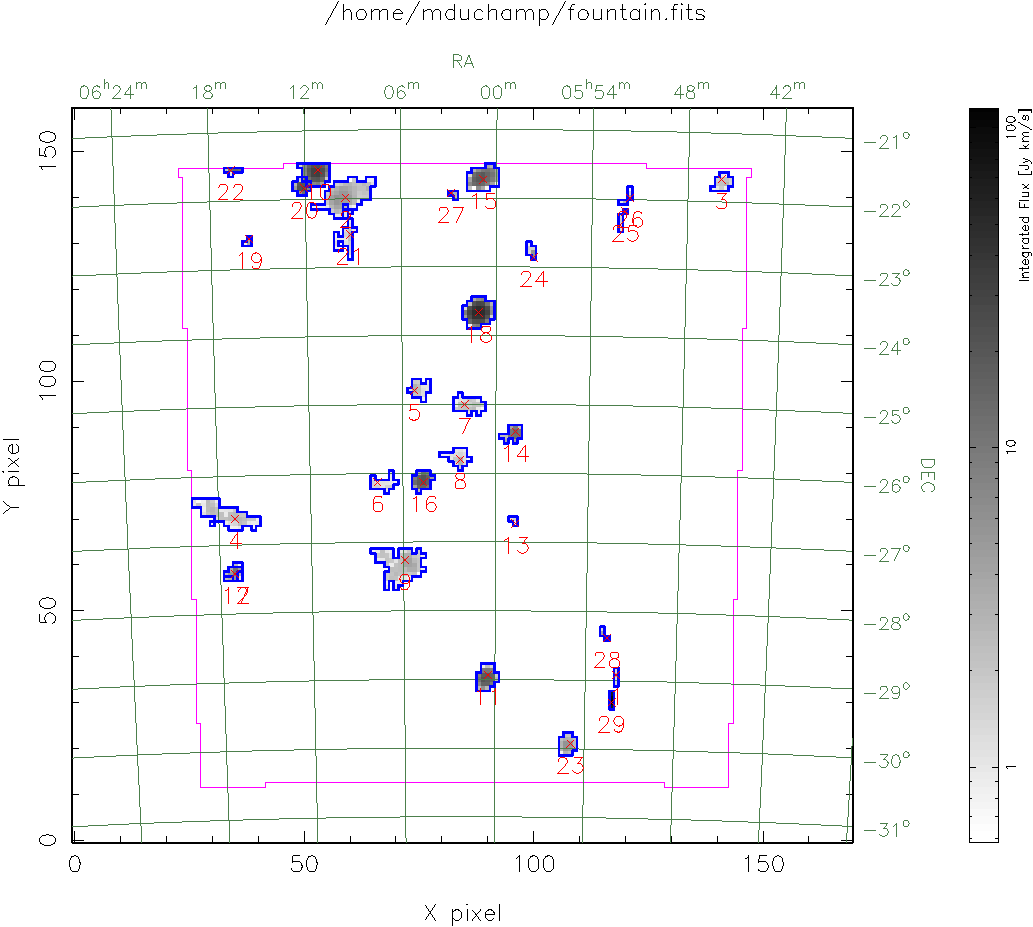
\includegraphics[width=\textwidth]{example_moment_map}
  \end{center}
  \caption{\footnotesize An example of the moment map created by
    \duchamp. The full extent of the cube is covered, and the 0th moment
    of each object is shown (integrated individually over all the
    detected channels). The purple line indicates the limit of the
    non-BLANK pixels.}
  \label{fig-moment}
\end{figure}

Additionally, two types of spatial images are optionally produced: a
combined 0th-moment map of the cube, combining just the detected
channels in each object, showing the integrated flux in grey-scale;
and a ``detection image'', a grey-scale image where the pixel values
are the number of channels in which that spatial pixel is
detected. These detections include pixels that are subsequently
discarded (due to the minimum-size criteria). In both cases, if
\texttt{drawBorders = true}, a border is drawn around the spatial
extent of each detection, and if \texttt{drawBlankEdges = true}, the
purple line dividing BLANK and non-BLANK pixels (as described above)
is drawn. An example moment map is shown in Fig.~\ref{fig-moment}.
The production or otherwise of these images is governed by the
\texttt{flagMaps} parameter.

The moment map is also displayed in a PGPlot XWindow (with the
\texttt{/xs} display option). This feature can be turned off by
setting \texttt{flagXOutput = false} -- this might be useful if
running \duchamp on a terminal with no window display capability, or
if you have set up a script to run it in a batch mode.

If the input image is one-dimensional, such a spatial map is not
possible. Instead, the detection map becomes a detection
spectrum. This shows the full spectral range, indicating (as for the
spectral plots above) the detection and growth thresholds, as well as
the `Milky Way' range and every detection that appears in the final
catalogue. It also indicates all pixels that were detected, including
those subsequently discarded, by thick black lines above the
spectrum. An example can be see in
Fig.~\ref{fig-1D-detection-spectrum}. Again, this plot is also
displayed in a PGPlot XWindow.

\begin{figure}[!t]
  \begin{center}
    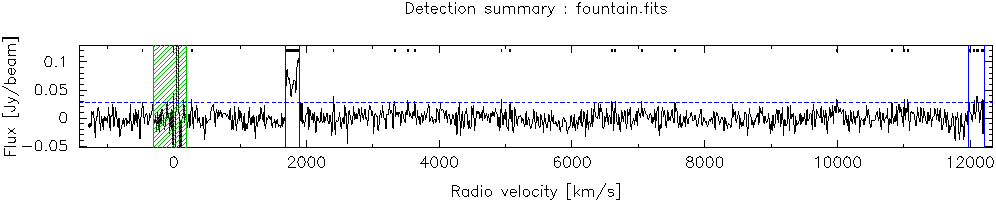
\includegraphics[width=\textwidth]{example_detection_spectrum}
  \end{center}
  \caption{\footnotesize An example of the one-dimensional detection
    spectrum plot, indicating detected sources and detected pixels,
    including those subsquently discarded due to the minimum-size
    criteria. The detection threshold is low to show the effect of
    detecting lots of single-pixel channels, which are then discarded,
    leaving just the two detections delimited by the blue lines.}
  \label{fig-1D-detection-spectrum}
\end{figure}



The purpose of these images is to provide a visual guide to where the
detections have been made, and, particularly in the case of the moment
map, to provide an indication of the strength of the source. In both
cases, the detections are numbered (in the same sense as the output
list and as the spectral plots), and the spatial borders are marked
out as for the cutout images in the spectra file. Both these images
are saved as postscript files (given by the parameters
\texttt{momentMap} and \texttt{detectionMap} respectively), with the
latter also displayed in a \textsc{pgplot} window (regardless of the
state of \texttt{flagMaps}).

\secB{FITS output}

\secC{Moment map}
\label{sec-momentOut}

The moment map described above can also be written to a FITS file, so
that it can be examined more closely, and have annotation files
overlaid. This works in the same way as for the mask image. To create
the FITS file, set the input parameter
\texttt{flagOutputMomentMap=true}. The file will be named according to
the \texttt{fileOutputMomentMap} parameter, or, if this is not given,
\texttt{image.MOM0.fits} (where the input image is called
\texttt{image.fits}).

\secC{Mask images}
\label{sec-maskOut}

It is also possible to write the mask array to a FITS file, for use in
other forms of post-processing. This array is designed to indicate the
location of detected objects. The value of the detected pixels is
determined by the input parameter \texttt{flagMaskWithObjectNum}: if
\texttt{true}, the value of the pixels is given by the corresponding
object ID number; if \texttt{false}, they take the value 1 for all
objects. Pixels not in a detected object have the value 0. To create
this FITS file, set the input parameter
\texttt{flagOutputMask=true}. The file will be named according to the
\texttt{fileOutputMask} parameter, or, if this is not given,
\texttt{image.MASK.fits} (where the input image is called
\texttt{image.fits}).

A spatial mask, or moment-0 mask, can also be written. This is simply
a two-dimensional image that shows which spatial pixels are detected
in one or more channels. Unlike the full mask file above, detected
pixels can only be recorded as 1 (as a given spatial pixel may appear
in multiple objects) -- that is, the parameter
\texttt{flagMaskWithObjectNum} does not affect the moment-0 mask. To
create this FITS file, set the input parameter
\texttt{flagOutputMomentMask=true}. The file will be named according
to the \texttt{fileOutputMomentMask} parameter, or, if this is not
given, \texttt{image.MOM0MASK.fits} (where the input image is called
\texttt{image.fits}).

\secC{Smoothed or Reconstructed image}
\label{sec-reconOut}

As discussed in \S\ref{sec-reconIO}, the reconstructed array, its
residual, or the smoothed array can be saved to a FITS file. This
allows examination of them offline, as well as their re-use by
\duchamp to save the expense of re-calculating. This behaviour is
controlled by \texttt{flagOutputRecon}, \texttt{flagOutputResid} and
\texttt{flagOutputSmooth}. Consult \S\ref{sec-reconIO} for further
details.

\secB{Re-examining previous \duchamp results}
\label{sec-reuse}


\secC{Binary Catalogue}

It is often the case that the bulk of the work in a \duchamp run is in
the searching for sources. If you are interested in re-doing some of
the spectral plots, or re-parameterising with different
\texttt{spectralType} settings, then having to re-run the searching
can be a bit off-putting. 

A solution to this problem exists in the ability to save a binary
catalogue, containing the information on the individual pixels
detected in each object. This is sufficient to recreate a set of
detections and re-do the parameterisation. To enable this mode, set
\texttt{flagWriteBinaryCatalogue=true}, and provide a filename with
\texttt{binaryCatalogue} (or use the default of
\texttt{duchamp-Catalogue.dpc}). The following will be written to the
catalogue: 
\begin{itemize}
\item Version of \duchamp. If it is not the same version, a warning is raised.
\item Current date and time.
\item The parameter set. Only the parameters affecting the
  pre-processing and searching are stored. Those related to, say,
  graphical output are not.
\item The measured statistics.
\item The pixels of each detected object, written using the run-length
  encoding described in \S\ref{sec-scan}.
\end{itemize}
These are written in binary format to conserve disk space, and are
sufficient to recreate the state of \duchamp after the searching has
taken place. 

To re-use this catalogue, set the flag \texttt{usePrevious=true} and
provide the binary catalogue filename via
\texttt{binaryCatalogue}. The catalogue will be loaded, and (provided
it loads correctly) the preprocessing and searching steps will be
skipped. The post-processing (\ie plotting and catalogue output) steps
will occur as normal, using the settings provided in the input
parameter file.

Note that while at this stage this is the only use for the binary
catalogues, it is anticipated that other functionality will be
provided in future - for instance, to allow conversion into mask
images. The binary catalogues are seen as a compact way of storing the
results of a \duchamp run. 

\secC{Selection of objects}

When re-running \duchamp on a previously-generated catalogue, it is
possible to produce the plots for only a selection of objects. Use the
\texttt{objectList} parameter to specify a set of objects, listing
individual object numbers or ranges, for example ``1,3-6,9,11'' means
objects 1,3,4,5,6,9,11. The output plots will be appropriately
modified: the spectral plots will only show these objects; the moment
map plot will only show the contribution from these objects; the
detection map will show the outlines of only these objects, although
all detected pixels are still shown in greyscale. 

Note that the object numbers here are valid for the catalogue as
sorted according to the \texttt{sortingParam} specification in the
parameter file. If you change this, the order of the catalogue may
change and the specific objects selected by \texttt{objectList} will
differ. 

This option is designed for the case of re-using a catalogue, but can
be used for a blind search as well. Of course, you may not know what
numbers the sources will turn out to be.

%%% Local Variables: 
%%% mode: latex
%%% TeX-master: "Guide"
%%% End: 
